\artigofalse
\chapter{R-package spsann: Optimization of Sample Configurations using Spatial 
Simulated Annealing}
\label{apen:spsann}

% 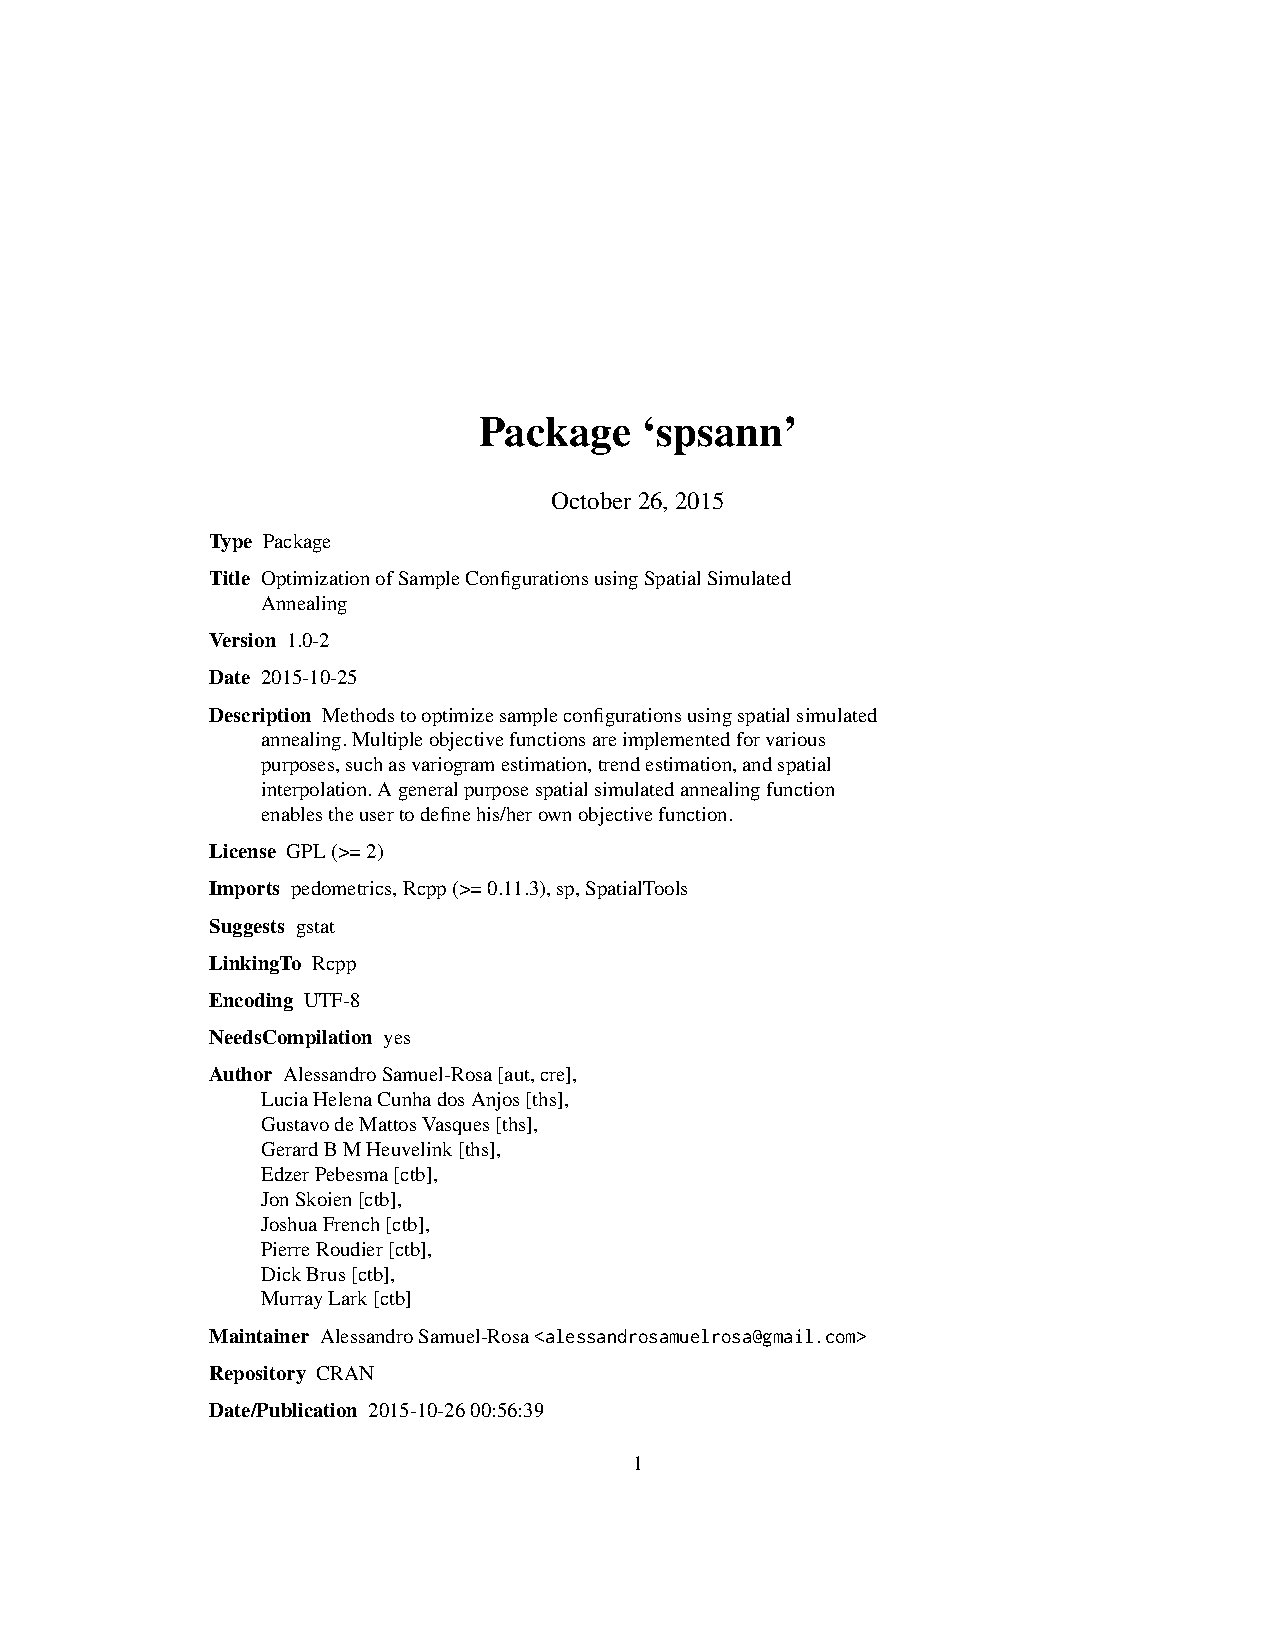
\includepdf[pages=-,pagecommand={}]{chap/spsann.pdf}

\section{Objective functions}

\subsection{Spatial trend identification and estimation}

CORR and DIST

\subsection{Variogram identification and estimation}

PPL: points and pairs; minimum and distribution

\subsection{Spatial interpolation}

MKV and MSSD

\subsection{Multi-objective optimization}

ACDC: CORR and DIST;
CLHS;
SPAN: CORR, DIST, PPL, and MSSD;

\section{Generation mechanism}

The \textit{generation mechanism} corresponds to the set of formal rules used 
to randomly perturb the sample configuration to create a new solution out of the
current one. This is done by adding random noise to the coordinates of one of 
the sample points, a process known as \textit{jittering}.

Before we jitter a given sample point, we have to define the maximum quantity 
of random noise that can be added to its coordinates, i.e. the area within 
which it can be moved around. In principle, this area corresponds to a rectangle
centred at the sample point that ignores the presence of non-sampling areas 
(e.g. buildings and water bodies) and the finiteness of the sampling region. We 
call this the \textit{neighbourhood}.

Once we know the size of the neighbourhood, we have to decide upon how much 
noise will be added to the coordinates of our sampling point, i.e. to choose a
candidate location in the neighbourhood. This can be done in two different ways.
We can use an \textit{infinite} set of candidate locations, that is, any 
location in the neighbourhood can be selected as the candidate location for our 
sample point. After a candidate location is selected, we check if it falls 
within the sampling region but does not fall within a non-sampling area. These 
checks usually are computationally demanding, the reason why this method is not 
implemented in the \textbf{spsann}-package.

A more efficient way of selecting a candidate location is to first identify the
set of \textit{effective} candidate locations for our sample point in the 
neighbourhood. This can be done using a \textit{finite} set of candidate 
locations. A finite set of candidate locations is created by discretizing the 
sampling region beforehand, that is, creating a fine grid of points that serve 
as candidate locations during the entire search for the optimum sample 
configuration. This is the least computationally demanding jittering method 
because, by definition, the candidate location will always fall within the 
sampling region and out of non-sampling areas.

Using a finite set of candidate locations has two main disadvantages. First, not
all locations in the sampling region can enter the sample. The sample points are
limited to a finite set of regularly spaced candidate locations which is not 
guaranteed to include the \textit{true} global optimum sample configuration. 
Second, when a sample point is jittered, it may be that the selected candidate 
location already is occupied by a sample point. When this happens, another 
candidate location has to be sought in the neighbourhood because we cannot have 
more than one sample point in the same location. In the worst case, most (or 
all) candidate locations in the neighbourhood are already occupied by a sample 
point -- in general, the more points there are in the sample (or the smaller 
the size of the neighbourhood (see bellow), the more likely it is that the 
selected candidate location already is occupied by a sample point. If a 
candidate location is not found, our sample point is kept in its original 
location.

The \textbf{spsann}-package uses a more elegant method based on using a finite
set of candidate locations coupled with a form of \textit{two-stage random 
sampling} as implemented in the \texttt{spsample}-function of the 
\textbf{spcosa}-package \citep{WalvoortEtAl2010}. The fine grid of points that 
cover the sampling region can be understood as being the centre nodes of a 
finite set of grid cells (or pixels of a raster image). In the first stage, one 
of the candidate 'grid cells' is selected with replacement in the neighbourhood,
i.e. independently of already being occupied by another sample point. The 
candidate location for our sample point is selected in the second stage within 
that 'grid cell' by simple random sampling. This method guarantees that a sample
 point can be placed at \textit{almost} any location within the sampling region.
It also discards the need to worry if the candidate location already is occupied
by a sample point, possibly speeding up the computations.

In order to increase its computational efficiency, the \textbf{spsann}-package 
uses a decrement function to reduce the size of the neighbourhood as the search
for the optimum sample configuration evolves. The reason for this is that, as 
the search evolves and approaches its end, it is likely that moving a sample 
point over a short distance contributes more to finding the global optimum than 
moving it over larger distances \citep{GroenigenEtAl1998}. The decrement 
function determines that the size of the neighbourhood is reduced linearly at 
the end of each chain $k_i$,

\begin{equation}
  x_{max} = x_{max\,0} - k_i / k * x_{max\,0} - x_{min} + x_{dim}

  y_{max} = y_{max\,0} - k_i / k * y_{max\,0} - y_{min} + y_{dim}
\end{equation}

where $x_{max}$ and $y_{max}$ are the dimensions of the neighbourhood in the 
next chain, i.e. the maximum allowed shifts in the x- and y-coordinates, 
$x_{max\,0}$ and $y_{max\,0}$ are the dimensions of the neighbourhood in the 
first chain, $x_{min}$ and $y_{min}$ are the minimum required shifts in the x- 
and y-coordinates, $x_{dim}$ and $y_{dim}$ are the grid spacings in the x- and 
y-coordinates, i.e. the grid cell size, and $k$ is the total number of chains.
The default settings stablish that the size of the neighbourhood in the first
chain is equal to half the maximum distance in the x- and y-coordinates of the
entire sampling region, and that the minimum jitter is equal to zero, i.e. that
the grid cell were the sample point is located can be selected as well. With 
these settings, at the end of the search, the neighbourhood will be constrained 
to the set of nine grid cells composed of that in which the sample point falls
and its eight surrounding grid cells.

\section{Annealing schedule}

The \textit{annealing schedule} corresponds to a set of formal rules that 
determine how the probability of accepting inferior sample configurations is 
decreased as the search for the globally optimum sample configuration evolves.

